\documentclass[11pt,a4paper]{article}
\usepackage{times}
\usepackage[german,english]{babel}
\usepackage[T1]{fontenc}
\usepackage[latin1]{inputenc}
%\selectlanguage{german}

\usepackage[numbers]{natbib}
%\usepackage{subfig}
\usepackage{subfigure}

\usepackage[pdftex]{graphicx}
\pdfcompresslevel=9

\parindent0em
\parskip1ex

\title{RoboCup Rescue Virtual Robots:\\Wireless Simulation Server Documentation}
\author{Max Pfingsthorn\\\texttt{\small m.pfingsthorn@jacobs-university.de}}
\date{\today}
\begin{document}

\DeclareGraphicsExtensions{.jpg,.pdf,.mps,.png}

\maketitle

\section{Introduction}

The purpose of the Wireless Simulation Server (WSS) is to simulate wireless network links in a disaster setting. The current version of the WSS does not implement a very accurate signal degradation model. However, it does force participants to deal with the main issues of wireless links, such as limited range and the resulting need for either multi-hop routing or temporary autonomous behavior.

The server works by acting as a hub for communication between the robots. During the competition, all data must be communicated through the Wireless Simulation Server.

Each entity (robot or operator station) that wants to transmit data via the WSS has to open a control connection to it. The proper protocol for communication via that connection is explained below. Only this connection is used to send and receive simulation specific commands and data. All other communication between entities that is facilitated by the WSS follows standard TCP/IP protocols.

A sketch of the process of connecting to another robot is presented below:
\begin{enumerate}
	\item Robot \emph{A} opens control connection to WSS and registers with a port it is listening on.
	\item Robot \emph{B} does the same.
	\item Robot \emph{A} queries the WSS for the port to connect to on the address the WSS is running on in order to have the WSS forward data to Robot \emph{B}.
	\item Robot \emph{A} connects with a standard TCP socket to the returned port.
	\item The WSS accepts the connection only if Robot \emph{B} is in range and opens another socket to the port Robot \emph{B} indicated it is listening on.
	\item Robot \emph{B} accepts the connection from the WSS.
	\item (Optional) In order to find out the name of the connecting entity, Robot \emph{B} queries the WSS with the \emph{remote port number} of the connection it just accepted.
\end{enumerate}

Both robots can send data via this established connection. The WSS will read up to 2048 bytes at a time from each robot if available and forward the exact same data to the other side. As all connections are implemented as their own threads that use \texttt{select} to poll for readable data, bandwidth should not be a problem.

\textbf{Important:} When running the WSS, be sure to turn off your firewall. The WSS chooses random ports to listen on. Also be sure to allow a connection to the port your robot is listening on.

\section{GUI}

Figure~\ref{fig:screenshot} shows the GUI. By default, the WSS will start listening on port 50000. If another port is desired, it can be changed in the top text field. Below is a box to choose the signal degradation implementation, the \emph{PropagationModel} (See section \ref{sec:PropagationModel}). The default \emph{NoopPropagationModel} always allows all connections, returning a signal strength of 0 dBm for any distance. This is mainly intended for testing purposes. Other implementations might be configurable, in which case the ``Configure'' button would be enabled.

\begin{figure}[htb]
	\centering
	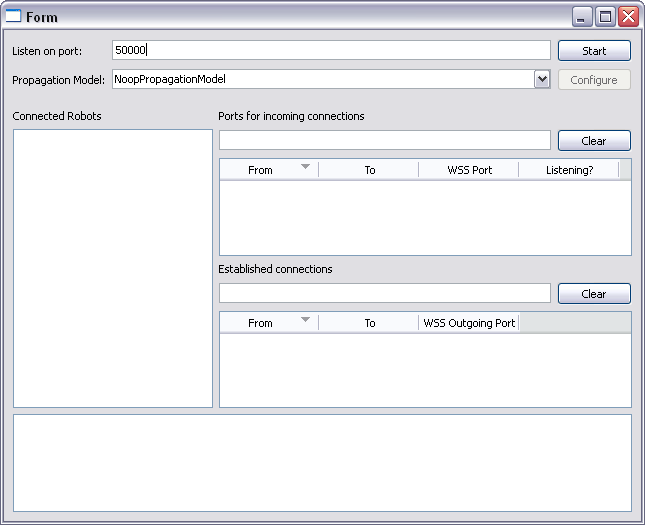
\includegraphics[width=.9\textwidth]{WSS-GUI.png}
	\caption{A screenshot of the version 0.1 GUI.}
	\label{fig:screenshot}
\end{figure}

The ``Connected Robots'' field shows an up-to-date list of robots that are currently registered with the WSS.

``Ports for incoming connections'' shows a list of connection to port mappings returned by the \texttt{DNS} query defined in Section \ref{sec:DNS}. If a certain connection was requested and a port allocated before, the ``Listening?'' field shows if this connection is currently allowed by the \emph{PropagationModel}. If this field shows \emph{false}, the WSS has closed this port temporarily to prevent robots from connecting.

``Established connections'' shows a list of currently active connections. Here, it also shows the port number used to connect to the second robot.

Both of the previous fields can be searched. By typing in the text fields above them, the lists will be filtered. To clear the search, press the ``Clear'' button.

The box below is a log window. Most of the actions performed in the background are documented here for debugging purposes.

\section{The Control Connection}

The WSS employs a control connection with each entity to support its operation. This connection is used to 
\begin{enumerate}
	\item register an entity with a port it is listening on,
	\item get the signal strength between two registered entities,
	\item get a port number on the WSS machine in order to connect to a different entity, and
	\item query which other entity connected given the originating port number,
\end{enumerate}

Registered entities are from here on called \emph{clients} of the WSS.

For each operation, clients are referenced by name used to identify their corresponding instances in the simulator. For example, if a robot was spawned in USARSim using the command

\texttt{INIT \{ClassName P2AT\} \{Name Robot1\} ... }

the corresponding WSS client name is also \texttt{Robot1}.

Just as with USARSim, all command strings and replies are terminated with a carriage return followed by a newline. In C escape sequences, this is equal to the string ``$\backslash$r$\backslash$n''.

There will always be a reply from the server. Specific error situations are included below. If a general error occurs, such as you sent a message which was not recognized, the server will respond with an \texttt{ERROR} message:

\texttt{ERROR \{Reason \textit{SomeReason}\}}

The reason is always a string without whitespace.

\subsection{Client Registration}

You \textbf{must} register your client before calling any other command. Also, you can only call this command once per connection request.

The command to initially register the identity of a connecting client is:

\texttt{INIT \{Robot \textit{RobotName}\} \{Port \textit{PortNumber}\} }

Optionally, the \textit{PortNumber} may also be a comma separated list of port numbers without whitespace. I.e.:

\texttt{INIT \{Robot \textit{RobotName}\} \{Port \textit{PortNumber1,PortNumber2}\} }

All following operations will use the given name. Incoming connections will be forwarded to the specified port(s) on the client's machine. If you try to register a name already in use, an error message will be sent. If successful, the server will reply:

\texttt{INITREPLY \{Status OK\}}

\subsection{Getting the Signal Strength}

Getting the signal strength between the current (i.e. set by \texttt{INIT}) robot and another is done via the command:

\texttt{GETSS \{Robot \textit{OtherRobotName}\} }

The reply of the server will be:

\texttt{SS \{Robot \textit{OtherRobotName}\} \{Strength \textit{SignalStrength}\}}

where \texttt{\textit{SignalStrength}} is a double formatted as text, \textit{NaN} if the \texttt{\textit{OtherRobotName}} is unknown, or \textit{INF} if the name is the same as given in the \texttt{INIT} command.

\subsection{Connecting to Another Station}
\label{sec:DNS}

In order to connect to another robot (or the operator), you need the port number on the WSS machine for this exact connection. Each port the WSS listens on is for exactly one pairing of robots or the operator. Actually, the WSS listens on two ports for each pairing, one for each direction. The WSS will match the IP address of the connecting client with the one used for the current control connection to the expected client for a minimum of security.

To get the port WSS is listening on for you (the robot specified in \texttt{INIT}) to connect to any other station in the simulated wireless network, use:

\texttt{DNS \{Robot \textit{RobotName}\}}

Optionally, you may add a field to the \texttt{DNS} message to ask for a connection to a specific port on the named robot:

\texttt{DNS \{Robot \textit{RobotName}\} \{Port \textit{OtherRobotPortNumber}\}}

The reply from the server will be:

\texttt{DNSREPLY \{Robot \textit{RobotName}\} \{Port \textit{PortNumber}\}}

where \textit{PortNumber} is the port on the WSS machine you should connect to. If the current signal strength is above a predefined threshold, the port will be open, listening for connections. If not, the port will be closed.

If the \textit{RobotName} given in the query doesn't exist, is the same as given in \texttt{INIT}, or the desired robot does not listen on the requested port, the \textit{PortNumber} will be \texttt{-1}. Additionally, the message will include a field called \texttt{Error} with a reason to distinguish these cases:

\texttt{DNSREPLY \{Robot \textit{RobotName}\} \{Port -1\} \{Error \textit{Reason}\}}

\subsection{Asking which Robot is Trying to Connect}

Since all incoming connections to the port specified in \texttt{INIT} originate from the WSS, it is important to be able to distinguish between different robots trying to connect. For that purpose, the WSS implements a reverse DNS lookup.

\texttt{REVERSEDNS \{Port \textit{PortNumber}\}}

queries the WSS for the name of the robot trying to connect given the originating port number on the WSS machine. This port number can be read from the socket with the C system call \texttt{getpeername()} in Unix and Windows. There are equivalents in all major programming languages.

On success, the WSS will reply:

\texttt{REVERSEDNSREPLY \{Port \textit{PortNumber}\} \{Robot \textit{RobotName}\}}

If the given port number is not in use, or used for a connection to another robot than given in \texttt{INIT}, the reply will be:

\texttt{REVERSEDNSREPLY \{Port \textit{PortNumber}\} \{Error UnknownOrIllegalPort\}}

\section{Making the Connection}

Actually connecting to another robot is very straightforward once the corresponding port has been queried from the WSS. This process uses plain sockets which are available on any programming platform.

Once a socket has been connected to the corresponding port on the WSS machine, you are free to use it as you please. Any form of data sent over the connection will be read from the incoming socket on the WSS and written straight to the outgoing one connected to the target robot.

If the signal strength should fall below some predefined threshold, both incoming and outgoing connections will simply be closed. The WSS will also stop listening for new connection attempts while the signal strength is too low. As soon as the signal strength is up again, the WSS will start listening on the same port as before, and reconnection will be possible again.

\section{Propagation Models}
\label{sec:PropagationModel}

\subsection{Introduction}

\emph{Propagation Models} implement a way to compute the signal attenuation between two connecting stations.
The main way to extend the WSS is by implementing new \emph{Propagation Models} as plugins.

Implementations of the main \emph{PropagationModel} interface communicate with the main WSS via the \emph{RobotLinkModel} interface, which allows the \emph{PropagationModel} to terminate and resume connections between two robots, kick out robots from the WSS by name, e.g. after their battery is empty, or get a list of currently registered robots.

In turn, the \emph{PropagationModel} allows the main WSS to query for the current signal strength between two robots and whether a connection between two given robots is currently possible. Also, the interface of the \emph{PropagationModel} is designed to allow the implementation to be multi-threaded and includes methods to stop and start the underlying implementation. Configurations have to be checked in the start method such that incomplete settings can be detected before the main WSS starts. Configurable implementations can also override methods to display a configuration dialog.

\subsection{\emph{NoopPropagationModel}}

The most basic implemented model is the \emph{NoopPropagationModel}. It always shows a signal strength of 0 dBm (i.e. no attenuation) for all connections. This is useful for debugging your network implementation without having to run USARSim at the same time.

\subsection{\emph{DistanceOnlyPropagationModel}}

The \emph{DistanceOnlyPropagationModel} implements the calculation of signal strength based on the distance between two robots in the simulator. It maintains a connection to the simulator to update the positions of robots continuously.

The signal strength is computed given a number of configurable parameters:

\begin{itemize}
	\item $S_c$: The signal cutoff in $dBm$. This is usually $-93$ as it is a physical property of the wireless channel. In the configuration dialog, this is referred to as ``Cutoff''.
	\item $P_{d_0}$: The path loss in $dBm$ at $d_0$ meters from the source.
	\item $d_0$: The distance from the source at which the path loss in $P_{d_0}$ is reached.
	\item $N$: The attenuation factor of the environment. This parameter decides how fast the signal is attenuated over distance.
\end{itemize}

The complete equation to compute the path loss at a certain distance $d_m$ from the source of the signal is:
\[
	S = P_{d_0} - 10 \cdot N \cdot \log_{10} \left(\frac{d_m}{d_0}\right)
\]

When $S$ falls below $S_c$, the \emph{DistanceOnlyPropagationModel} will terminate any connections between the two robots in question and also stop the threads listening on the ports which correspond to this robot pair. This means that subsequent attempts to connect to a robot which is out of range will fail with a ``Connection refused'' error since that port is no longer open on the WSS. Once $S$ is high enough again, e.g. after the robots moved closer together, the ports will be opened again for new connections.

\begin{figure}[htb]
	\centering
		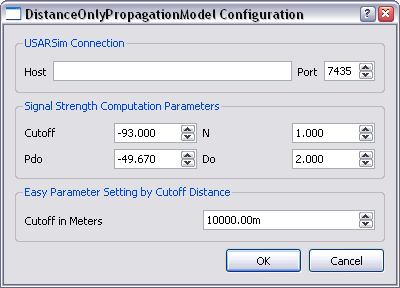
\includegraphics[width=.8\textwidth]{WSS-DistanceOnlyConfig.png}
	\caption{The configuration dialog for the \emph{DistanceOnlyPropagationModel}.}
	\label{fig:DistanceOnlyPropagationModel-Config}
\end{figure}

Figure~\ref{fig:DistanceOnlyPropagationModel-Config} shows the configuration dialog for this propagation model. The first section configures the connection parameters to USARSim. Here, it is especially important to know the right port. \textbf{Do not use port 3000}, which is the standard port to connect to for spawning robots and getting sensor data. Port 7435 is the standard port to use here. You must type in a numerical IP address, the WSS does not resolve DNS names.

The middle section allows the configuration of the computation parameters mentioned above. While it is possible to change the ``Cutoff'' parameter ($S_c$ above), it is recommended to leave it at $-93dBm$.

The last section facilitates changing the desired distance at which the \emph{DistanceOnlyPropagationModel} terminates connections. Any changes in the above parameters is immediately reflected here. Also, changing the desired distance here will automatically update the parameter $N$ above.

Once OK is clicked, the parameter values are saved in the \emph{DistanceOnlyPropagationModel}. It also saves these settings persistently on your computer. In Windows, this is done via the Registry. This way, your previous settings are available again the next time you start the WSS.

\subsection{Future Implementations}

Future implementations include but are not limited to:
\begin{itemize}
	\item \emph{RayTracingPropagationModel}: A method which runs ray traces in the simulator to detect the number of obstacles between two entities in order to attenuate the signal more accurately.
\end{itemize}

Other implementations, such as a debugging one, which allows to selectively break connections between specific entities is also possible.

\section{License}

The application and this documentation is released under the GNU General Public License (GPL) version 2.

\end{document}